\documentclass[12pt]{article}
% load the necessary packages

\usepackage[paperheight=9in,paperwidth=13.24in,margin=0in]{geometry}
\usepackage[dvipsnames,prologue,table]{pstricks}
\usepackage{pst-text}
\usepackage{pst-char}
\usepackage{pst-grad}
\usepackage{graphicx}
\usepackage{lipsum}


% begin the document and suppress page numbers
\begin{document}

\pagestyle{empty}
% create the box with the front cover picture
\newsavebox\IBox
\sbox\IBox{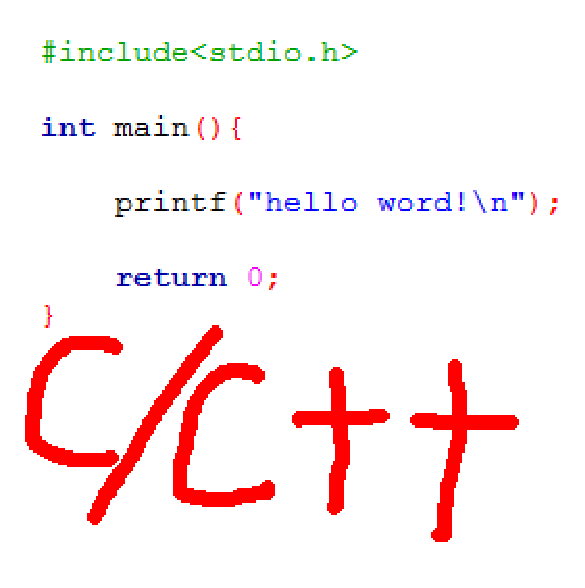
\includegraphics[height=9in]{front.eps}}
% set up the picture environment
\psset{unit=1in}
\begin{pspicture}(13.24in,9in)
% set up the fonts we use

\DeclareFixedFont{\PT}{T1}{ppl}{b}{it}{0.5in}
\DeclareFixedFont{\PTsmall}{T1}{ppl}{b}{it}{0.4in}
\DeclareFixedFont{\PTsmallest}{T1}{ppl}{b}{it}{0.3in}
\DeclareFixedFont{\PTtext}{T1}{ppl}{b}{it}{11pt}
\DeclareFixedFont{\Logo}{T1}{pbk}{m}{n}{0.3in}
% create a maroon background

\psframe[fillstyle=solid,fillcolor=Maroon](0,0)(13.24,9)


% place the front cover picture
\rput[lb](7.24,0){\usebox\IBox}
% put the text on the front cover
\rput[lb](7.74,7){\PT \color{white}{Secrets of the Stamen}}
\rput[lb](8.94,6){\PTsmall \color{white}{Yuri Robbers}}
\rput[lb](9.04,0.8){\PTsmallest \color{white}{Lughdunum Press}}
% put the text on the spine (note the rotation over 270 degrees)
\rput[l]{270}(6.62,8.5){\PTsmall%
\color{white}{Yuri Robbers --- Secrets of the Stamen}}
% put the publisher’s logo on the spine
\rput[b](6.62,0.75){\color{white}{\fbox{\Logo L}}}
% Create a Box containing the text for the back cover



\newsavebox\Blurbbox
\sbox\Blurbbox{\begin{minipage}{4.5in}
\textcolor{white}{\lipsum[1]}
\end{minipage}}
% And position the box
\rput[tl](1,8){\usebox\Blurbbox}
% Then we close all open environments
\end{pspicture}
\end{document}
